\documentclass[12pt, titlepage]{article}

\usepackage{booktabs}
\usepackage{tabularx}
\usepackage{hyperref}
\usepackage{graphicx}
\usepackage{multirow}
\hypersetup{
    colorlinks,
    citecolor=black,
    filecolor=black,
    linkcolor=red,
    urlcolor=blue
}
\usepackage[round]{natbib}
\usepackage[normalem]{ulem}

%% Comments

\usepackage{color}

\newif\ifcomments\commentstrue %displays comments
%\newif\ifcomments\commentsfalse %so that comments do not display

\ifcomments
\newcommand{\authornote}[3]{\textcolor{#1}{[#3 ---#2]}}
\newcommand{\todo}[1]{\textcolor{red}{[TODO: #1]}}
\else
\newcommand{\authornote}[3]{}
\newcommand{\todo}[1]{}
\fi

\newcommand{\wss}[1]{\authornote{blue}{SS}{#1}} 
\newcommand{\plt}[1]{\authornote{magenta}{TPLT}{#1}} %For explanation of the template
\newcommand{\an}[1]{\authornote{cyan}{Author}{#1}}

%% Common Parts

\newcommand{\progname}{ProgName} % PUT YOUR PROGRAM NAME HERE
\newcommand{\authname}{Team \#, Team Name
\\ Student 1 name and macid
\\ Student 2 name and macid
\\ Student 3 name and macid
\\ Student 4 name and macid} % AUTHOR NAMES                  

\usepackage{hyperref}
    \hypersetup{colorlinks=true, linkcolor=blue, citecolor=blue, filecolor=blue,
                urlcolor=blue, unicode=false}
    \urlstyle{same}
                                


\begin{document}

\title{User Guide\\Greenway} 
\author{Team \#11, Roadkill
		\\ Bilal Zaki - shaikb2 
		\\ Jash Mehta - mehtaj8
		\\ Pranay Kotian - kotianp 
        \\ Priyansh Shah - shahp36
        \\ Sharjil Mohsin - mohsis2
        \\ Utsharga Rozario - rozariou
}
\date{\today}

\maketitle

\pagenumbering{roman}

\tableofcontents

\newpage

\section{Revision History}

\begin{tabularx}{\textwidth}{p{3cm}p{2cm}X}
\toprule {\bf Date} & {\bf Version} & {\bf Notes}\\
\midrule
April 5, 2023 & 1.0 & Revision 0\\
\bottomrule
\end{tabularx}

\section{Symbols, Abbreviations and Acronyms}

N/A

\newpage

\pagenumbering{arabic}

\section{Introduction}
Greenway is a web application that allows you to calculate the most fuel efficient route between two locations. As gas prices continue to rise, it becomes increasingly more important to be mindful of how much money you spend on gas. This user guide is meant to help you become acquainted with the Greenway application and all of it's features. Included are instructions for typical use cases as well as answers to frequently asked questions. 

\section{Definitions}
Greenway: our program\\
Interface: the front-end of our application\\
Mileage: a number of kilometres traveled or covered\\
Road grade: the slope of the road\\


\section{Getting Started}

The Greenway interface was designed to be simple, efficient, and self explanatory. The right side of the screen displays the map. The left side of the screen contains all the user input fields. 

\begin{center}
  \makebox[\textwidth]{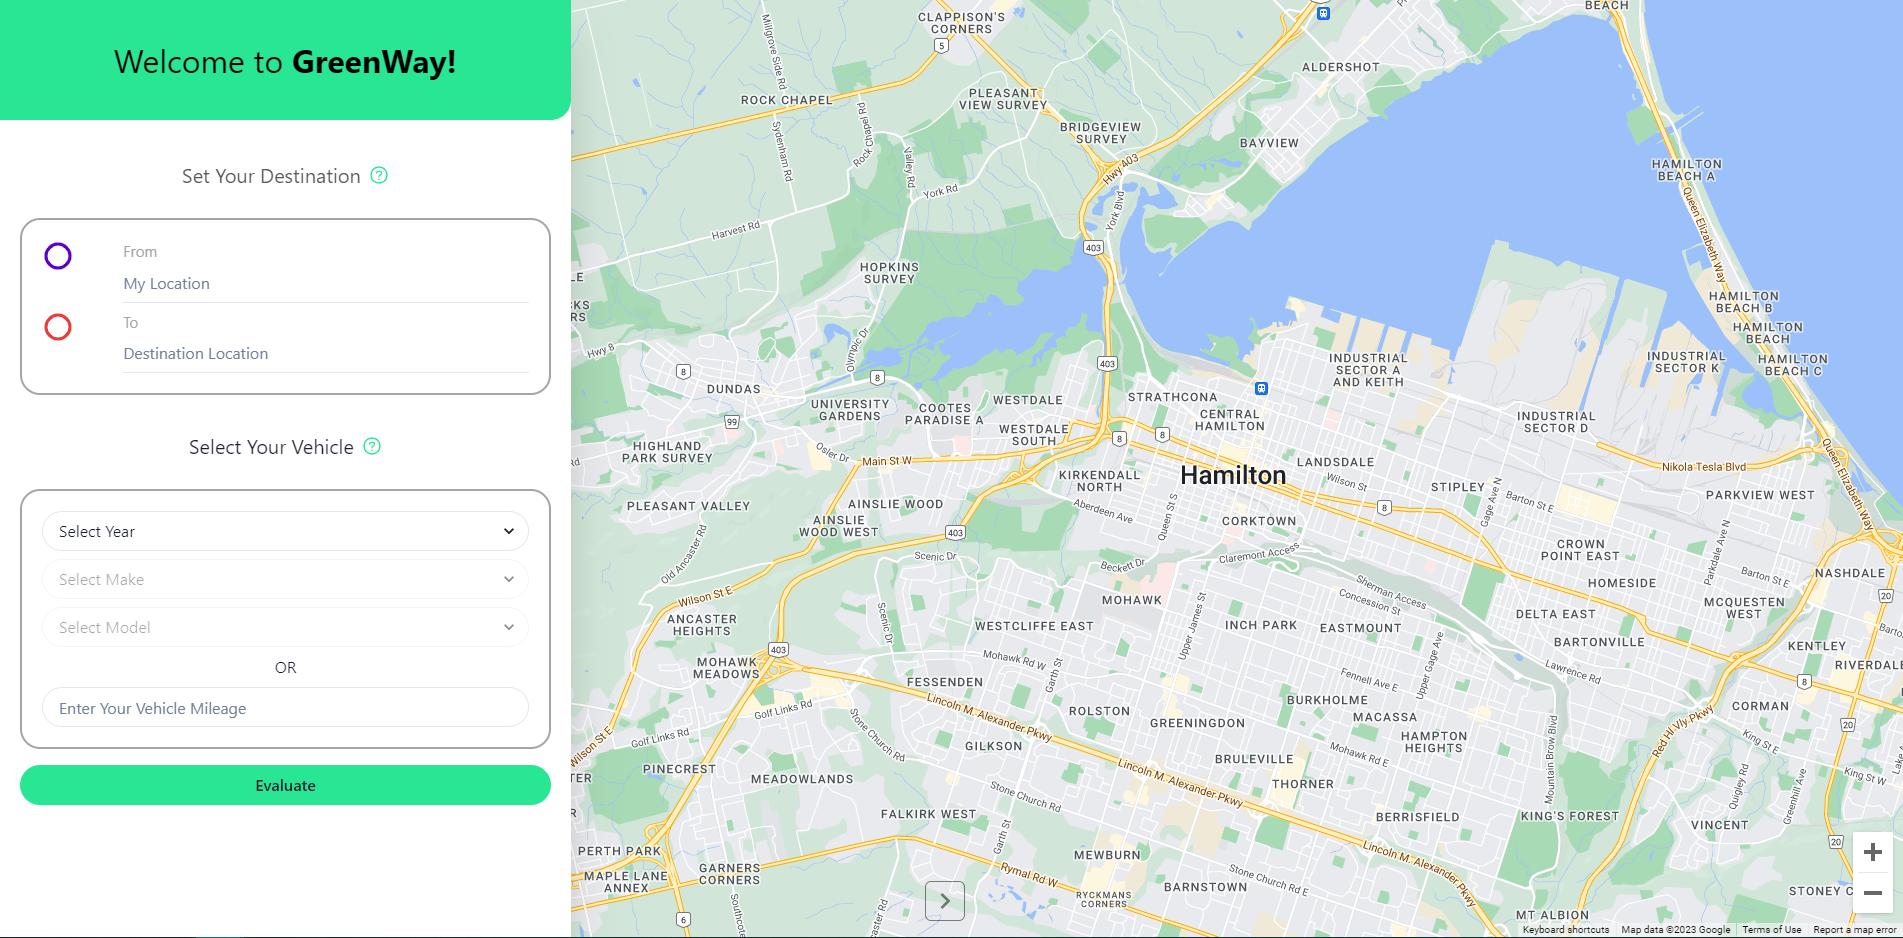
\includegraphics[width=\linewidth]{images/landing-page.png}}
\end{center}

The first section has input fields for your starting location and ending location (destination). 

\begin{center}
  \makebox[\textwidth]{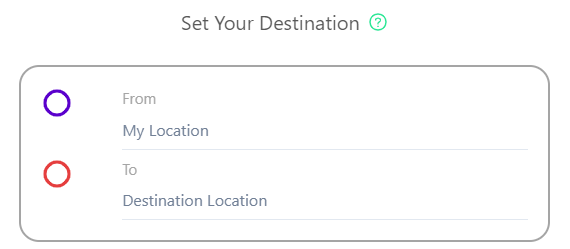
\includegraphics[width=\linewidth]{images/section1.png}}
\end{center}

The second section has input fields for your vehicle information. You can either enter the year, make, and model of your car, or you can enter the specific mileage of your vehicle. If you enter the year, make, and model of your car, Greenway will search up the estimated mileage for that vehicle in our database. 

\begin{center}
  \makebox[\textwidth]{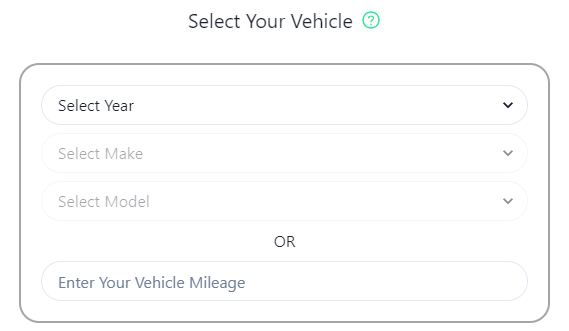
\includegraphics[width=\linewidth]{images/section2.png}}
\end{center}

Once you have entered your location and vehicle information, press evaluate to calculate the most fuel efficient route. Greenway will display the mileage, gas prices, distance, and total cost of the trip after a few seconds. 

\begin{center}
  \makebox[\textwidth]{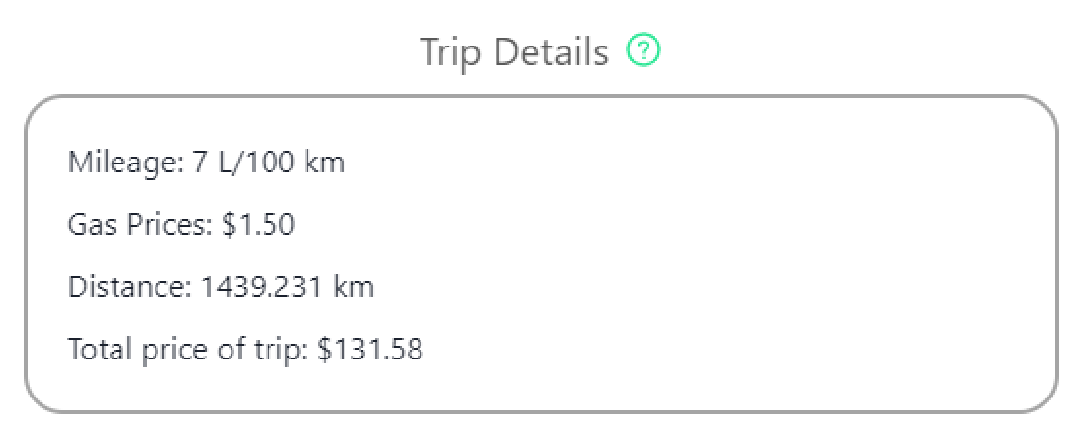
\includegraphics[width=\linewidth]{images/total-cost.png}}
\end{center}

\section{Troubleshooting}
\subsection{Trip Details Not Updating}
Sometimes the app will display zeroes for all the trip details or it will display the last trip's price - in this case wait a few seconds for the app to respond.

\subsection{Vehicle Not Available in Database}
You can enter vehicle mileage if your car is not available in the application. 

\section{Frequently Asked Questions}

\subsection{Will Greenway store any information that I have inputted into the application?}
Any information inputted by the user will not be stored 

\subsection{Do I need to input my trip start and destination typo-free?}
No, if you were to make a typo while entering the beginning and end of your journey, our system will use the top most relevant Google Maps search result related to your input, so small typos may be tolerated and produce a route.

\subsection{Do I need to install anything to run Greenway?}
No, Greenway is a simple web application that can be run on any modern browser. The application can be run on any device with access to the internet once it will be hosted on a server (however mobile support is currently limited).

\subsection{How does Greenway calculate my fuel consumption?}
Using a database that contains over 27000 cars, we are able to determine the fuel economy of the vast majority of cars in Canada by their city and highway efficiency, and use that information along with an optimized mapping algorithm to determine the most fuel efficient route. With this, we take into account the changes in elevation along the route (for example, a more uphill route leads to more fuel consumption dependent on the road grade), and the cheapest gas station along the route to accurately determine real-time gas prices and ensure our users get accurate information on their fuel cost.

\end{document}